\documentclass{article}

\include{stddefs}
\include{imodefs}

\chapterno{2}

\begin{document}

\chapter{Linear equations}

Modern mathematical terminology may seem abstract, but a lot of it comes from
equation solving. We will talk about linear equations in this chapter to
motivate the concept of matrices in the next chapter.

Linear equations are equations, where the unknowns
only appear to the first power. For example,
$x^2 + x + 1 = 0$ is not a linear equation in the unknown $x$, since $x$ to the second power ($x^2$) appears in the equation,  whereas
$2 x - 3 = 1$ is.
We may also consider several linear equations with several unknowns, such as
\begin{align}
x + y + z &= 3\\
x - y + z &= 1\\ \label{eqstart}
x + y - z &= 1
\end{align}

consisting of three linear equations with the three unknowns $x$, $y$ and $z$.

\beginshex
Try to come up with a solution to \eqref{eqstart} i.e., find
numbers $x, y, z$ satisfying all three equations. Do not use a computer.
Is there more than one solution?

Write down two linear equations with two unknowns, which do not
have a solution.
\endshex

Do the exercise above, before you evaluate the Sage code below, which uses
the dreaded solve function. The solve function should always be used as a last resort.

\begin{sage}
x, y, z = var('x, y, z')
solve([x+y+z == 3, x - y + z == 1, x + y - z == 1],
x, y, z)
\end{sage}



\section{One linear equation with one unknown}

Very simple rules apply when solving linear equations.

Consider as an example the linear equation $2 x - 3 = 1$ in the unknown $x$.
Solving this equation amounts to reducing to an expression $x=$ a number. This
is called \emph{isolating} $x$. The process is very mechanical:
\begin{align*}
2 x - 3 &= 1\\
&\Updownarrow\\
2 x - 3 + 3 &= 1 + 3\\
&\Updownarrow\\
2 x &= 4\\
&\Updownarrow\\
\left(\frac{1}{2}\right) 2 x &= \left(\frac{1}{2}\right) 4\\ 
&\Updownarrow\\
x &= 2
\end{align*}
If you look closely, you will see that we have used the rules
\begin{align*}
&a=b\qquad \iff \qquad a + c = b + c\\
&a=b\qquad \iff \qquad t a = t b,
\end{align*}
where $a, b, c$ are numbers and $t$ is a number $\neq 0$.

\beginshex
Point out the mistake(s) in the \footnote{argument}{This teaser was presented at the workshop for new teaching assistants, August 2020.} below showing that $2 = 1$.
\begin{align*}
  a &= b \iff \\
  a^2 &= a b \iff\\
  a^2 - b^2 &= a b - b^2 \iff \\
  (a + b)(a - b) &= b (a - b) \iff\\
  a + b &= b \iff \\
  2 b &= b \iff \\
  2 &= 1.
\end{align*}
\endshex

\begin{quizexercise}[showhide]
\begin{quiz}
\question
A saline solution is a mixture of $0.9$\% sodium chloride in water. Suppose that you have
$2$ liters of water containing $9$\% sodium chloride. How many liters of
distilled water ($0$ percent sodium chloride)
do you need to add to get a saline solution.
\answer{F}
$4.5$ liter
\answer{F}
$10$ liter
\answer{T}
$18$ liter
\end{quiz}
\end{quizexercise}

\beginshex
Diophantus's youth lasted $1/6$ of his life. He grew a beard after $1/12$ more. After $1/7$ more
he got married. Five years later he had a son. The son lived half as long as the father
and Diophantus died four years after the son. At what age did Diophantus die?

\begin{hideinbutton}{Link/Hint}
  You can read about Diophantus and the solution to the puzzle in the \url{Wikipedia entry}{https://en.wikipedia.org/wiki/Diophantus} about him. Please
  try solving the problem on your own first.
\end{hideinbutton}
\endshex


\section{Several linear equations with several unknowns}

The linear equation $2 x - 3 = 1$ has only one unknown with the unique solution
$x=2$. \emph{If one linear equation has more than one unknown, then it has
  infinitely many solutions}. Consider as an example the linear equation
$2 x - 3 y = 1$ with the unknowns $x$ and $y$.
Using the procedure as before, we get
\begin{align*}
2 x - 3 y &= 1\\
&\Updownarrow\\
x &= \frac{1}{2} + \frac{3}{2} y
\end{align*}
Here we are free to choose $y$ in infinitely many ways giving
infinitely many solutions $(x, y)\in \RR^2$.

\subsection{Several equations}

Several equations with several unknowns also make sense. Consider
\begin{align*}
x + y &= 3\\
2 x - 3 y &= 1
\end{align*}
Two numbers $x$ and $y$ form a solution $(x, y)\in \RR^2$ if both equations are satisfied.
From the example above, we know that 
\begin{equation}\label{isol}
x = \color{blue}{\frac{1}{2} + \frac{3}{2} y}. 
\end{equation}
This can be inserted for $x$ in the first equation and we get
$$
3 = x + y = \color{blue}{\frac{1}{2} + \frac{3}{2} y} + y = \frac{1}{2} + \frac{5}{2} y.
$$
Here we end up with one linear equation in one variable $y$.
The solution is $y=1$, which is inserted in the equation \eqref{isol} giving
$x = 2$. Therefore the solution to the equations is $(x, y) = (2, 1)$.

\begin{quizexercise}[showhide]
\begin{quiz}
  \question
  \url{Kona coffee}{https://en.wikipedia.org/wiki/Kona_coffee} is a delicacy priced at $200$ kroner for $400$ grams.
  A standard $500$ gram bag of Arabica beans is priced at $60$ kroner.

  A merchant wishes to mix coffee beans of these sorts aiming for a price of
  $75$ kroner for $400$ grams. Which one of the percentages below
  comes closest to the content of Kona coffee in the mixture?
  
\answer{T}
$18\%$
\answer{F}
$5\%$
\answer{F}
$30\%$
\answer{F}
$12\%$
\end{quiz}
\end{quizexercise}


\section{Gauss elimination}

When solving systems of several linear equations, it is natural to
fix one of the equations, isolate an unknown and then insert
in the other equations.

Let us study this procedure focusing on an example with
two equations and three unknowns:
\begin{align*}
x + 2 y + z &= 8\\
2 x + y + z &= 7
\end{align*}
In the first equation we isolate $x = 8 - 2 y - z$, which is then inserted into the second
equation:
$$
2 x + y + z = 2(8 - 2 y - z) + y + z = - 3 y - z + 16 = 7 \implies -3 y - z = -9. 
$$
It makes perfect sense to multiply the first equations by $2$ and subtract from the second
equations. This operation gives
$$
-3 y -  z = -9.
$$
It is not a coincidence that these two operations give the same result.


\begin{theorem}\index{Gauss elimination}
Suppose that  
\begin{align*}
a_1 x_1 + a_2 x_2 + \cdots + a_n x_n &= c_1\\
b_1 x_1 + b_2 x_2 + \cdots + b_n x_n &= c_2
\end{align*}
are two linear equations in the unknowns $x_1, \dots, x_n$ with
$a_1\neq 0$. The equation gotten by first isolating
$x_1$ in the first equation and then inserting in the second equation
is identical to the equation you get by adding the first equation multiplied 
by $-b_1/a_1$ to the second equation.
\end{theorem}
\begin{proof}[showhide]
  Isolating $x_1$ in the first equation inserted in the second equation gives
  the equation
\begin{equation}\label{equ1}
b_1\left(\frac{c_1}{a_1} - \frac{a_2}{a_1} x_2 - \cdots -\frac{a_n}{a_1} x_n\right) + b_2 x_2 + \cdots + b_n x_n = c_2
\end{equation}
Adding $-b_1/a_1$ multiplied to the first equation to the second equation gives
\begin{equation}\label{equ2}
\left(b_2 - \frac{b_1 a_2}{a_1}\right) x_2 + \cdots +
\left(b_n - \frac{b_1 a_n}{a_1}\right) x_n = c_2 - \frac{b_1}{a_1} c_1
\end{equation}
Using basic arithmetic you can see that \eqref{equ1} can be rewritten to
\eqref{equ2}. 
\end{proof}


Multiplying an equation by a number and then adding to another equation
is easier to handle than the method of isolating and inserting. We have
showed above that they produce the same result. Below is
an extended example.


\begin{example}[showhide]
We wish to solve the system of equations

\begin{equation}\label{origlign}
\begin{matrix}
&2 x &+ &y &+ &z &= 7\\
&x &+ &2y &+ &z &= 8\\
&x &+ &y &+ &2 z &= 9
\end{matrix}.
\end{equation}


The first step is subtracting the third equation from the second:
$$
\begin{matrix}
&2 x &+ &y &+ &z &= 7\\
&x &+ &2y &+ &z &= 8\\
&x &+ &y &+ &2 z &= 9
\end{matrix}\quad\iff
\begin{matrix}
&2 x &+ &y &+ &z &= 7\\
& &  &y &- &z &= -1\\
&x &+  &y &+ &2 z &= 9
\end{matrix}
$$
Then we multiply the third equation by $2$ and subtract from the first:
$$
\begin{matrix}
&2 x &+ &y &+ &z &= 7\\
& &  &y &- &z &= -1\\
&x &+  &y &+ &2 z &= 9
\end{matrix}
\quad\iff
\begin{matrix}
& &-  &y &- &3 z &= -11\\
& &  &y &- &z &= -1\\
&x &+  &y &+ &2 z &= 9
\end{matrix}
$$
Finally we add the second equation to the first:
$$
\begin{matrix}
& &-  &y &- &3 z &= -11\\
& &  &y &- &z &= -1\\
&x &+  &y &+ &2 z &= 9
\end{matrix}\quad\iff
\begin{matrix}
& &  & &- &4 z &= -12\\
& &  &y &- &z &= -1\\
&x &+  &y &+ &2 z &= 9
\end{matrix}
$$
We have now reduced the original system of equations \eqref{origlign} to
$$
\begin{matrix}
& &  & &- &4 z &= -12\\
& &  &y &- &z &= -1\\
&x &+  &y &+ &2 z &= 9
\end{matrix},
$$
where the first equation shows that $z = 3$. Now $z = 3$ can be inserted into
the second equation, giving $y - 3 = -1$, which is solved by $y=2$.
Finally 
$y = 2$ and $z=3$ are inserted into the third equations giving the equation
$x + 8 = 9$, which is solved by $x=1$.

One very important observation here is that $x=1, y=2$ and $z=3$ is the only
solution to  \eqref{origlign}. This is a logical consequence of the
bi-implication arrows $\iff$ throughout the above calculations.

\begin{sage}
x, y, z = var('x, y, z')
solve(
[2*x+y+z == 7,
x + 2*y + z == 8,
x + y + 2*z == 9],
x, y, z)
\end{sage}

\end{example}




The elimination or substitution method for solving systems of linear equations
is old and well known.
\url{Sir Isaac Newton}{https://en.wikipedia.org/wiki/Isaac_Newton} described in $1720$
the methods eloquently as follows.

\begin{quote}
  \emph{And you are to know, that by each Æquation one unknown Quantity may
  be taken away, and consequently, when there are as many Æquations
  and unknown Quantities, all at length may be reduc'd into one, in
  which there shall be only one Quantity unknown.}
\end{quote}


The mathematical rockstar \url{Carl Friedrich
  Gauss}{https://en.wikipedia.org/wiki/Carl_Friedrich_Gauss} used the method
to determine the orbit for the asteroid
\url{Pallas}{https://en.wikipedia.org/wiki/2_Pallas}. The mathematical analysis
of the observations lead him to the famous \url{least squares method}{https://en.wikipedia.org/wiki/Least_squares} and
a system of six linear equations with six unknowns.

The method is known today by the term \emph{Gaussian elimination} even though Gauss
was not the first to introduce it. In fact it appeared already in \emph{The Nine Chapters
  on the Mathematical Art}, which is an ancient Chinese mathematics book compiled over several
centuries from the 10th century BCE to the 2nd century CE. This book contains
several practical problems and their solutions. An example is
\begin{quote}
  There are three categories of corn. Three bundles of the first class,
  two of the second and one of the third make $39$ measures. Two of the
  first, three of the second, and one of the third make $34$ measures. Finally
  one of the first, two of the second and three of the third make $26$ measures.
  How many measures of graín are contained in one bundle of each class?
\end{quote}


\begin{quizexercise}[showhide]
 \begin{quiz}
\question
How many solutions does the system of equations below have?
\begin{align*}
x + y + z &= 0\\
x - y + z &= 0\\
x + y - z &= 0
\end{align*}
\answer{F}
None.
\answer{T}
Precisely one.
\answer{F}
Infinitely many.
\end{quiz}
\end{quizexercise}


\begin{quizexercise}[showhide]
How many solutions does the system of equations below have?
  \begin{quiz}
\question

\begin{align*}
x + y + z &= 0\\
x - y + z &= 0\\
5 x + y +5z &= 0
\end{align*}
\answer{F}
Precisely one.
\answer{F}
Precisely two.
\answer{T}
Infinitely many.
\end{quiz}
\end{quizexercise}

\beginshex
Find the solutions to
$$
\begin{matrix}
& x &+ &3 y &+ &z &= &2\\
&-2 x &- &5 y &+ &3 z &= &4.
\end{matrix}
$$
by expressing $x$ and $y$ in terms of $z$ i.e., isolate $x$ on the
left hand side, such that
\begin{align*}
  x &= \dots\\
  y &= \dots,
\end{align*}
where $\dots$ indicate an expression only in the unknown $z$.
\endshex


\beginshex
Your enemy transmits secret codes $(x_1, x_2, x_3, x_4)$ consisting of four integers $x_1, x_2, x_3, x_4$ over the internet. He does
not transmit the code itself but an encrypted version $(y_1, y_2, y_3, y_4)$ given by
\begin{equation*}
\begin{matrix}
  y_1 &= &2 x_1 &+ &x_2 &+ &3 x_3 &+  &4 x_4\\
  y_2 &= &x_1 &+ &2 x_2 &+ &3 x_3 &+  &4 x_4\\
  y_3 &= &3 x_1 &+ &3 x_2 &+ &x_3 &+  &x_4\\
  y_4 &= &4 x_1 &+ &4 x_2 &+ &2 x_3 &+  &3 x_4
\end{matrix}.
\end{equation*}
You have knowledge of the encryption method above and by listening in on
a recent communication, you learn that the encryption
$(15, 16, 12, 20)$ was sent. What was the original secret code before the encryption?

\begin{hideinbutton}{Extra credit}
  Suppose that you only know that the encryption scheme is
\begin{equation*}
\begin{matrix}
  y_1 &= &a_{11} x_1 &+ & a_{12} x_2 &+ &a_{13} x_3 &+  &a_{14} x_4\\
  y_2 &= &a_{21} x_1 &+ &a_{22} x_2 &+ &a_{23} x_3 &+  &a_{24} x_4\\
  y_3 &= &a_{31} x_1 &+ &a_{32} x_2 &+ &a_{33} x_3 &+  &a_{34} x_4\\
  y_4 &= &a_{41} x_1 &+ &a_{42} x_2 &+ &a_{43} x_3 &+  &a_{44} x_4
\end{matrix},
\end{equation*}
and that you have no knowledge of the numbers $a_{11}, \dots, a_{44}$.
How many transmissions do you need to know at the minimum to find
these encryption numbers?
\end{hideinbutton}

\endshex


\beginshex
The diagram below shows a network of roads and $6$ intersections.
Every road is labeled by a number indicating the average number
of cars per hour on the road. Some of these numbers 
$f_1, \dots, f_7$ are unknowns. Write up a system of linear
equations for finding $f_1, \dots, f_7$. 

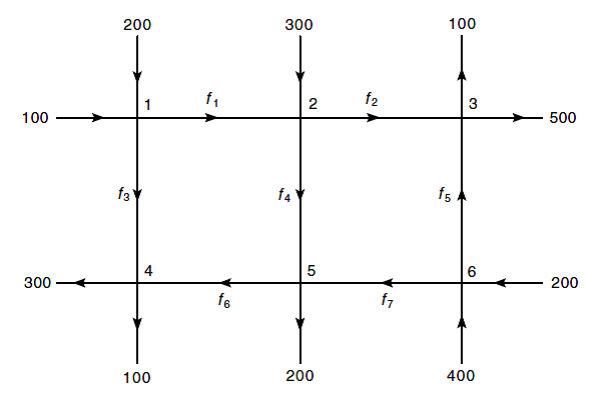
\includegraphics{trafik.png}


Compute
$f_1, f_2, f_3, f_4, f_5, f_6$ supposing that $f_1=200$ and $f_7=100$.
\endshex


\begin{example}\label{Googleprlineqs}

This example relates to the famous Google page rank algorithm.  

  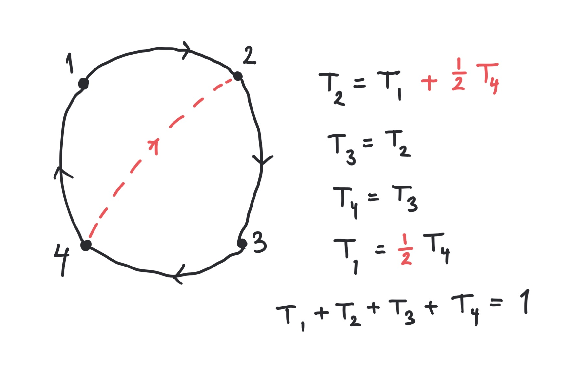
\includegraphics{pagerankgraph.png}


  Suppose we have a very simple internet with only four webpages
  as depicted above with arrows indicating that a webpage links to another.

  We wish to study traffic in this network in the sense that we let a random
  websurfer jump from a given webpage to another by selecting a link randomly.

  If you look at the network without the punctured red arrow, it is almost clear
  the a random websurfer will spend $25$ \% of the time uniformly in each of the
  four nodes.

  However, if we introduce the puntured red arrow, then the percentages in
  each node are given by the linear equations above. Here it turns out that
  website $1$ only gets around $14$ \% of the time (the other websites get double this time each).

\end{example}




\begin{hideinbutton}{Simulation of page rank in python}
You may try out the python code below to simulate a random tour
of the small internet in Example \ref{Googleprlineqs}.

\begin{sage}
import random

# Incidence matrix

A = [[0,1,0,0], [0,0,0,1], [1,1,0,0], [0,0,1,0]]

def neighbors(n):
    return [i for i, e in enumerate(A[n]) if e != 0]

def simulate(n, num): # Simulate random walk num times from node n in matrix A
    count = [0] * len(A)
    node = n
    count[n] = 1
    for i in range(num):
        node = random.choice(neighbors(node))
        count[node] += 1
    return count

simulate(0, 1000)        
\end{sage}

The list (or matrix)
\begin{code}
  A = [[0,1,0,0], [0,0,0,1], [1,1,0,0], [0,0,1,0]]
\end{code}
encodes the graph of links between the four nodes $0, 1, 2, 3$. From
$A$ you can see that $2$ links to $0$ and $1$ and that
$0$ links to $1$. The command

\begin{code}
  simulate(0, 1000)
\end{code}

simulates a random surf with $1.000$ clicks starting in node $0$.

The linear equations really seem to give the right result!
\end{hideinbutton}
  

\section{Polynomials}\label{section:polynomials}

Before going further into examples of linear equations we need to introduce (non-linear)
functions called \emph{polynomials}. A polynomial of degree $n$ is a function $f:\RR\rightarrow \RR$
of the form
\begin{equation}\label{poldef}
f(x) = a_n x^n + a_{n-1} x^{n-1} + \cdots + a_1 x + a_0,
\end{equation}
where $a_0, \dots, a_n$ are real numbers and $a_n\neq 0$. We call $a_0, \dots, a_n$
the \emph{coefficients} of $f$.
The degree of the polynomial $f$ is denoted
$\deg(f)$. As an example,
$$
x^3 - 2 x + 17
$$
is a polynomial of degree $3$ with
\begin{align*}
  a_3 &= 1\\
  a_2 &= 0\\
  a_1 &= -2\\
  a_0 &= 17.
\end{align*}

In addition to the polynomials defined in \eqref{poldef} with $a_n\neq 0$,
we also view the function $f(x) = 0$ as a polynomial, called the \emph{zero polynomial}.
The zero polynomial does \footnote{not}{All its coefficients are zero!} have a degree.

The set of all polynomials is denoted
$\RR[x]$, so that for example it makes sense to write
$$
x^2 - 5 x + 6\in \RR[x].
$$
It is probably the most natural functions from $\RR$ to $\RR$ you can come up with.
If you look at \eqref{poldef}, you will see that the output is formed by using
addition and multiplication (by $x$ and selected real numbers).



You can compute with polynomials treating the \emph{variable} $x$ as
a number. For example,
$$
(3 x^2 + 2 x + 1) (2 x + 1) = 6 x^3 + 7 x^2 + 4 x + 1.
$$
In general a polynomial of degree $m$ times a polynomial of degree $n$ is a
polynomial of degree $m+n$.


In the sage window below we encounter for the first time the \texttt{sympy} library. The
input format and commands for handling polynomials should be clear from the context.

\begin{sage}
from sympy import expand
from sympy.abc import x
f = 3*x**2 + 2*x + 1
g = 2*x + 1
expand(f*g)
\end{sage}


You have already seen polynomials
of degree one. They have the form
$$
f(x) = a x + b,
$$
where $a$ and $b$ are real numbers and $a\neq 0$. Similarly
polynomials of degree two are called quadratic polynomials. They look
like
$$
f(x) = a x^2 + b x + c,
$$
where $a, b$ and $c$ are real numbers and $a\neq 0$. 

To get a feeling for the behavior of polynomials you should experiment in the sage
window below. Try varying the degree and the coefficients of the polynomial in the plot.
Also adjust the plot interval for the right view.

\begin{sage}
  plot(x**4 - 10*x**3 + 35*x**2 - 50*x + 24, (x, 0.5, 4.5))
\end{sage}

\beginshex
Suppose that
$$
f(x) = a x^2 + b x + c.
$$
To compute $f(x)$ it seems that you need $3$ multiplications
($a\cdot x\cdot x$ and $b\cdot x$) and $2$ additions.
Can you compute $f(x)$ with only $2$ multiplications and $2$ additions?

Try to generalize to the computation of $f(x)$, where $f$ is a polynomial
$$
f(x) = a_n x^n + a_{n-1} x^{n-1} + \cdots + a_1 x + a_0,
$$
of degree $n$ (you should only need $n$ multiplications and $n$ additions here).
\endshex

\subsection{Polynomial division}

Division is sometimes referred to as long division when
focusing on the method for division. Let us look
at the situation for integers first.

The remainder of 
$14$ divided by $4$ is $2$, since
$$
14 = 3\cdot 4 + 2.
$$
Here the remainder $2$ is strictly less than the divisor $4$.

For polynomials we have a similar situation, where the degree
is taken into account. For example, the remainder of
$x^3 + x + 1$ divided by $x^2 + x + 1$ is $x+2$, since
\begin{equation}\label{poldiv}
x^3 + x + 1 = (x-1)(x^2 + x + 1) + (x+2).
\end{equation}
Here the degree of the remainder $1$ is strictly less 
than the degree of the divisor $2$.

The Python library \url{\texttt{sympy}}{https://www.sympy.org/} contains a
wealth of functions for symbolic mathematics. In the window
below, it is shown how the polynomial division \eqref{poldiv}
is computed using the
\url{Polynomial Manipulaton}{https://docs.sympy.org/latest/modules/polys/index.html} section
of the \texttt{sympy} documentation.

\begin{sage}
from sympy import div
from sympy.abc import x
div(x**3+x+1, x**2+x+1)
\end{sage}

The (division) algorithm for carrying out (long) division of
polynomials is explained by an example in the video below.

\begin{video}
\youtube{SLIEUcOwVxA}
\end{video}


\beginshex
Watch the five minute video above and
carry out (do not use a computer) the polynomial division alluded to in \eqref{poldiv}.
\endshex

The general result about division of polynomials is given below.

\begin{theorem}[emph]\label{poldivthm}
Let $d(x)\in \RR[x]$ be a non-zero polynomial. Then 
for every polynomial $f(x)\in \RR[x]$, there exists
polynomials $q(x), r(x)\in \RR[x]$, such that
\begin{equation}\label{identpol}
f(x) = q(x) d(x) + r(x),
\end{equation}
where $r(x) = 0$ or $\deg(r(x)) < \deg(d(x))$.
\end{theorem}
\begin{proof}[showhide]
We will prove this using induction on $n = \deg(f)$. Suppose that
$$
f(x) = a_n x^n + \cdots\qquad\text{and}\qquad d(x) = b_m x^m + \cdots
$$
In general if $\deg(d(x)) = m > n$, then
$$
f(x) = 0\cdot d(x) + f(x)
$$
satisfies the assumptions for the identity in \eqref{identpol} with
$ q(x) = 0$ and $r(x) = f(x)$.

If $m\leq n$, then $f(x) - a_n b_m^{-1} x^{n-m} d(x)$ is a polynomial of
degree $<n$. So by induction we may find polynomials $q_0(x)$ and $r_0(x)$, such that
$$
f(x) - a_n b_m^{-1} x^{n-m} d(x) = q_0(x) d(x) + r_0(x).
$$
Therefore
$$
f(x) = (q_0(x) + a_n b_m^{-1} x^{n-m})d(x) + r_0(x)
$$
giving the desired result with $q(x) = q_0(x) + a_n b_m^{-1} x^{n-m}$ and $r(x) = r_0(x)$. 
\end{proof}




\subsection{Roots of polynomials}

A real number $\alpha\in \RR$ is called a \emph{root} of the polynomial $f(x)\in \RR[x]$ if
$f(\alpha) = 0$. This is a very fundamental definition. It is mirrored beautifully in the following
result.

\begin{proposition}\label{proproot}
A real number $\alpha$ is a root of the polynomial $f(x)\in \RR[x]$ if and only if
$$
f(x) = q(x) (x-\alpha),
$$
for some polynomial $q(x)\in \RR[x]$.
\end{proposition}
\begin{proof}[showhide]
By Theorem \ref{poldivthm}, we may write
\begin{equation}\label{degonediv}
f(x) = q(x)(x-\alpha) + r(x),
\end{equation}
where $r(x)= 0$ or $r(x)$ is a non-zero polynomial of degree zero i.e., a  non-zero
constant. Now the result follows, since $f(\alpha) = q(\alpha)(\alpha - \alpha) + r(\alpha) = r(\alpha)$ 
using \eqref{degonediv}.
\end{proof}


\beginshex
Is there an easy way of deciding if a polynomial $d(x) = a x + b$ of degree one divides
a polynomial $f(x)$ without performing the (long) division of $f(x)$ by
$d(x)$. Here divides means that $f(x) = q(x) d(x)$ for some polynomial $q(x)$.
\endshex

A quadratic polynomial
$$
a x^2 + b x + c
$$
has at most two roots given
by the formula (one root for $+$ and one for $-$ in $\pm$ below)
\begin{equation}\label{formulaqe}
\frac{-b\pm \sqrt{b^2 - 4 a c}}{2 a},
\end{equation}
if its \emph{discriminant} $b^2 - 4 a c$ is $\geq 0$.

\begin{frameit}
  Deriving the formula \eqref{formulaqe} comes from a classical algebraic trick called \emph{completing the square}. Looking
  at the quadratic equation $a x^2 + b x + c = 0$, what bothers us is the term $b x$. If $b=0$ we could solve the equation rewriting to
  $$
  x^2 = -\frac{c}{a}
  $$
  and then taking square roots. The first step in this direction is rewriting
  the equation
  $$
  a x^2 + b x + c = 0
  $$
  to
  \begin{equation}\label{eqi}
  x^2 + \frac{b}{a} x = -\frac{c}{a}.
  \end{equation}
  We would like to add a number $d^2$ to both sides of \eqref{eqi} so that the left hand side comes to look like
  \begin{equation}\label{eqii}
    (x + d)^2 = x^2 + 2 x d + d^2.
  \end{equation}
    This is what is called completing the square.

  Comparing the left hand side of \eqref{eqi} with the right hand side of \eqref{eqii}, we find that 
  $$
  d = \frac{b}{2 a}
  $$
  works.
  Therefore \eqref{eqi} implies
  $$
  \left( x + \frac{b}{2a}\right)^2 = -\frac{c}{a} + \left(\frac{b}{2 a}\right)^2.
  $$
  This identity can be rewritten into the formula \eqref{formulaqe} for solving the
  quadratic equation.
  \end{frameit}


For polynomials of degree three (cubic
polynomials) there is a \url{formula}{https://en.wikipedia.org/wiki/Cubic_function#General_solution_to_the_cubic_equation_with_real_coefficients}, but these days nobody remembers it. Also for polynomials of
degree four (quartic polynomials) there is a \url{formula}{https://en.wikipedia.org/wiki/Quartic_function#Solution}. But for polynomials of degree five (quintic polynomials) and up, one can prove
that \url{a formula cannot exist}{https://en.wikipedia.org/wiki/Abel\%E2\%80\%93Ruffini_theorem}!

  An exceedingly important result is quoted and proved below: the degree of a polynomial is
  an upper bound for its number of roots.

  
\begin{theorem}[emph]\label{atmostn}
  A non-zero polynomial $f(x)\in \RR[x]$ of degree $n > 0$ can have at most $n$ roots.
\end{theorem}
\begin{proof}[showhide]
We will prove this by induction starting with $n = 1$. Here
$f(x) = a x + b$ for $a, b\in \RR[x]$ and
$$
f(\alpha) = 0\iff \alpha = - a^{-1} b.
$$
Therefore $f(x)$ has precisely one root. Suppose now that we have proved that
polynomials of degree $n$ has at most $n$ roots. Assume that 
$f(x)$ is a polynomial of degree $n + 1$. If $f(x)$ has no roots,
we are done with the proof. Suppose that $f(\alpha) = 0$ i.e.,
$\alpha$ is a root in $f$. Then
$$
f(x) = q(x) (x-\alpha)
$$
by Proposition \ref{proproot}. Here $q(x)$ has to be a polynomial of degree $n$ and
therefore by induction, $q(x)$ has at most $n$ roots. However, if $f(\beta) = q(\beta) (\beta - \alpha) = 0$,
then either $\beta = \alpha$ or $q(\beta) = 0$. We have proved that 
$f(x)$ cannot have more than $n+1$ roots.
\end{proof}


\begin{remark}\label{remarkatmostn}
  Theorem \ref{atmostn} has a few interesting consequences. First it implies that two
  identical polynomials i.e., $f(x) = g(x)$ for every $x\in \RR$ must have
  the same coefficients.

  Secondly if two polynomials $f(x)$ and $g(x)$ of degree $n$ satisfy
  $f(x_i) = g(x_i)$ for distinct points $x_1, \dots, x_{n+1}$, then
  $f(x) = g(x)$.
\end{remark}

\beginshex
In Remark \ref{remarkatmostn} it is stated that if two polynomials $f(x)$ and $g(x)$ of degree $n$ satisfy
  $f(x_i) = g(x_i)$ for distinct points $x_1, \dots, x_{n+1}$, then
  $f(x) = g(x)$. How does this follow from Theorem \ref{atmostn}?
\endshex

It might happen that a  polynomial of degree $n$ has precisely $n$ roots, but it could have less or
even no roots: the polynomials
$$
x^2 + 1, x^4 + 1, x^6 + 1, \dots
$$
have no roots, whereas for example
$$
x^2 - 2 x + 1
$$
is a quadratic polynomial with only one root. However polynomials of degree $1, 3, 5, \dots$ always have at 
least one root.

\begin{theorem}[emph]
A polynomial of odd degree always has a root.
\end{theorem}

The proof of this result is beyond our scope now and will have to wait for tools from analysis.

\beginshex
Compute the roots of the quartic
$$
x^4 - 5x^2 + 6.
$$
\endshex

\beginshex
Give an example of a polynomial of degree $17$ with precisely one root.
\endshex

\beginshex
Suppose that $\alpha, \beta$ are two roots of the quadratic polynomial
$$
f(x) = x^2 + b x + c.
$$
How can $b$ and $c$ be computed in terms of $\alpha$ and $\beta$?
Show concretely how this can be applied to the polynomial
$g(x) = x^2 - 5 x + 6$: if you know that $g(2) = 0$ how can you easily
find the other root?

\begin{hint}
Show that $f(x) = (x-\alpha)(x-\beta)$ and use this.  
\end{hint}
\endshex



\section{Applications to polynomials}


A line in the plane is given by its equation $y = a x + b$, where $a$ is the slope 
and $b$ is the intersection with the $y$-axis. Two lines in the plane
are either parallel or intersect in a single point.

\beginshex
The two lines $y = x+1$ and $y=-x+2$ have a single point
of intersection. Compute this point.

Give an example of two parallel lines and their equations.
\endshex

Through two (distinct) points $(x_1, y_1)$ and $(x_2, y_2)$ with $x_1\neq x_2$ passes a unique line 

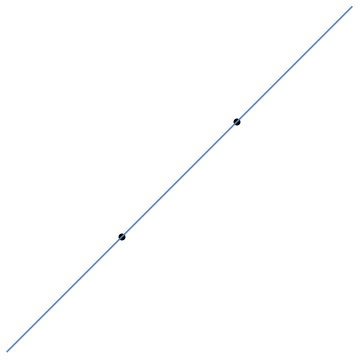
\includegraphics[width="50\%"]{linje.svg}

You can find the equation for this line by solving
two equations with two unknowns $a$ and $b$:
\begin{align*}
x_1 a + b &= y_1\\
x_2 a + b &= y_2
\end{align*}
We might as well apply Gauss elimination to solve this system. First we
subtract the second equation from the first. This gives
$(x_1 - x_2) a = y_1 - y_2$. Therefore
$$
a = \frac{y_1 - y_2}{x_1 - x_2}.
$$
Inserting this $a$ in the first equation we get
$$
b = \frac{x_1 y_2 -x_2 y_1}{x_1 - x_2}.
$$
We can also in a quite explicit way just write
\begin{equation}\label{lagrlin}
y = f(x) = y_1 \frac{x - x_2}{x_1 - x_2} + y_2 \frac{x - x_1}{x_2 - x_1}.
\end{equation}
The function $f(x)$ in 
\eqref{lagrlin} is a polynomial of degree one with
$f(x_1) = y_1$ and $f(x_2) = y_2$.


In almost the same way we may find a unique quadratic polynomial
$$
y = a x^2 + b x + c
$$
through three points $(x_1, y_1), (x_2, y_2)$ and $(x_3, y_3)$ with distinct $x$-values:

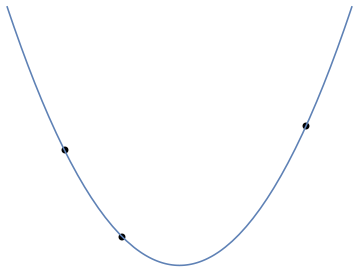
\includegraphics[width="50\%"]{parabel.svg}


Here we end up with three linear equations in the unknowns $a, b$ and $c$:
\begin{align}\label{lignpar}
x_1^2 a + x_1 b + c &= y_1\\
x_2^2 a + x_2 b + c &= y_2\\
x_3^2 a + x_3 b + c &= y_3
\end{align}
It is not immediately obvious that this system of equations has a solution. But watch the following trick evolve.

We may explicitly construct the quadratic polynomial passing through the three points as
\begin{align}\label{lagrpar}
  y = f(x) = &y_1 \frac{(x - x_2)(x-x_3)}{(x_1 - x_2)(x_1-x_3)} + y_2 \frac{(x - x_1)(x - x_3)}{(x_2 - x_1)(x_2-x_3)}\\
  &+ y_3 \frac{(x - x_1)(x - x_2)}{(x_3 - x_1)(x_3-x_2)}
\end{align}
Take a moment and verify that $f(x_1) = y_1, f(x_2) = y_2$ and $f(x_3)= y_3$. This also proves that
the system of equations in \eqref{lignpar} can be solved.

\begin{remark}
Notice in \eqref{lagrpar} that
$$
y = y_1 L_1(x) + y_2 L_2(x) + y_3 L_3(x),
$$
where (for example)  $L_1$ is a polynomial of degree two satisfying
$$
L_1(x_1)=1,\quad L_1(x_2)=0, \quad\text{and}\quad L_1(x_3)=0.
$$ 
What about $L_2$ and $L_3$ with respect to $x_1, x_2$ and $x_3$?
\end{remark}

\beginshex\label{lagrcol}
Compute the polynomial you get when you apply \eqref{lagrpar} to $x_1 = 1, x_2 = 2, x_3= 3$ and
$y_1 = 1, y_2 = 2, y_3 = 3$. How do you explain this result in terms of the
points $(x_1, y_1), (x_2, y_2)$ and $(x_3, y_3)$ plotted in plane?
\endshex


The natural generalization is that there exists a unique polynomial of degree $\leq n$ passing through $n+1$ points
$(x_1, y_1), \dots, (x_{n+1}, y_{n+1})$ with distinct $x$-values.

The rather miraculous trick above in \eqref{lagrpar} is called \url{Lagrange interpolation}{https://en.wikipedia.org/wiki/Lagrange_polynomial} and can be generalized to polynomials of arbitrary degree.
Below is an example of five points defining a unique polynomial of degree four.

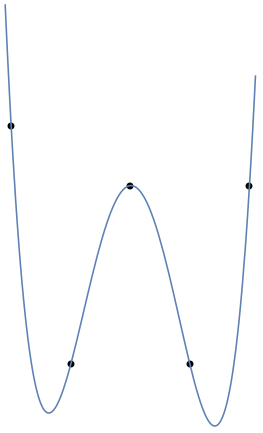
\includegraphics[width="35\%"]{quartic.svg}


\subsection{The magic of Lagrange polynomials}

Let us study the remarkable polynomial in \eqref{lagrpar} a little deeper: suppose we have $n$ numbers
\begin{equation}\label{Lpts}
x_1, x_2, \dots, x_n.
\end{equation}
Then these numbers give $n$ polynomials each of degree $n-1$:
$$
L_i(x) = \frac{1}{C_i} (x-x_1) \cdots (x-x_{i-1})(x-x_{i+1}) \cdots (x - x_n),
$$
where
$C_i = (x_i-x_1) \cdots (x_i-x_{i-1})(x_i-x_{i+1}) \cdots (x_i - x_n)$ for
$i = 1, \dots, n$.

The polynomial $L_i(x)$ is called the $i$-th
\url{Lagrange basis polynomial}{https://en.wikipedia.org/wiki/Lagrange_polynomial}
associated to the $n$ numbers $x_1, \dots, x_n$.
It satisfies
$L_i(x_1) = \cdots = L_i(x_{i-1}) = 0$, $L_i(x_i) = 1$ and
$L_i(x_{i+1}) = \cdots = L_i(x_n) = 0$ i.e., $L_i(x)$ is equal to zero
evaluated at all of the numbers $x_1, \dots, x_n$ except at $x_i$
where it evaluates to $1$.


The Lagrange basis polynomials allow us to construct a polynomial $f$ of degree $\leq n$ through
$n+1$ points $(x_1, y_1), \dots, (x_{n+1}, y_{n+1})$ i.e., a polynomial $f$ such that
\begin{align*}
  f(x_1) &= y_1\\
         &\vdots\\
  f(x_{n+1}) &= y_{n+1}
\end{align*}
simply as
$$
f(x) = y_1 L_1(x) + \cdots + y_{n+1} L_{n+1}(x).
$$
However, $f(x)$ does not have to have degree $n$. For example, it could come out as a line through
three points $(x_1, y_1), (x_2, y_2)$ and $(x_3, y_3)$ (see Exercise \ref{lagrcol}).

\beginshex
Compute $a_0, a_1, a_2, a_3\in \RR$ so that
\begin{align*}
f(-2) &= -1\\
f(-1) &= 1\\
f(1) &= 1\\
f(2) &= 1,
\end{align*}
where
$$
f(x) = a_0 + a_1 x + a_2 x^2 + a_3 x^3.
$$
You can do this either by Lagrange interpolation or by solving linear equations. Which one
do you prefer?
\endshex

\begin{example}

Can you predict the next number in the sequence starting with
\begin{equation}\label{csseq}
15,\quad 34,\quad 65,\quad 111,\quad 175,\quad 260,\quad 369?
\end{equation}

This question \footnote{was posed}{Thanks to Tobias Bendsen Poulsen for notifying me about this.} by the tutors in a class session for new computer science students. Let us put the sequence \eqref{csseq} inside a table like

$$
\def\arraystretch{1.5}
\begin{array}{c|ccccccc}
n & 1 & 2 & 3 & 4 & 5 & 6 & 7\\ \hline
f(n) & 15 & 34 & 65 & 111 & 175 & 260 & 369
\end{array},
$$

where $f:\NN\rightarrow \NN$ is the secret function responsible for the sequence. We would like to compute $f(8)$. Assuming that the $f(n)$ is a polynomial function, we may simply compute the unique polynomial of  degree $\leq 6$ through the $7$ points
$$
(1, 15),\quad (2, 34),\quad (3, 65),\quad (4, 111),\quad (5, 175),\quad (6, 260),\quad (7, 369).
$$

We know how to do this either by solving linear equations or computing with Lagrange polynomials. It turns out that Sage has built in functions helping us here.

\begin{sage}
R = PolynomialRing(QQ, 'x')
f = R.lagrange_polynomial([(1, 15), (2, 34), (3, 65), (4, 111), (5, 175), (6, 260), (7, 369)])
f(8)
\end{sage}

Press the button to see what next number is in the sequence (computed using the secret polynomial). See also the
description of \url{Neville's algorithm}{https://en.wikipedia.org/wiki/Neville\%27s_algorithm} in Wikipedia for an easier approach to
computing $f(8)$.


\end{example}

\section{Shamir secret sharing}

Lagrange interpolation is used in cryptography in \url{Shamir's secret sharing}{https://en.wikipedia.org/wiki/Shamir\%27s_Secret_Sharing}. Secret sharing is important in many practical situations. Here is an example quoted from Wikipedia:
  \begin{quote}
    A company needs to secure their vault's passcode. They could
    encrypt it, but what if the beholder of the secret key is
    unavailable or turns rogue?

    One needs to distribute the secret. This is where SSS comes in. It
    can be used to encrypt the vault's passcode and generate a certain
    number of shares, where a certain number of shares can be
    allocated to each executive within the company. Now, only if they
    pool their shares can they unlock the vault. The threshold can be
    appropriately set for the number of executives, so the vault is
    always able to be accessed by the authorized individuals. Should a
    share or two fall into the wrong hands, they couldn't open the
    passcode unless the other executives cooperated.
  \end{quote}

  The mathematics that takes care of this is surprisingly simple. Suppose the secret is the
  number $a_0$. Then we construct the polynomial
  \begin{equation}\label{sss}
  f(x) = a_0 + a_1 x + a_2 x^2 + \cdots + a_m x^m
  \end{equation}
  for some other numbers $a_1, \dots, a_m$.  We know that this
  polynomial is uniquely given by its values in $m+1$ distinct numbers
  (see Remark \ref{remarkatmostn}). So if there are $n$ trusted people
  we could distribute the shares
  $$
  (1, f(1)), (2, f(2)), \dots, (n, f(n))
  $$
  to them. Here we suppose that $n > m$. In this setting, if there are less than $m+1$ of
  the people present they cannot open the vault. If $m+1$ or more people are present they
  can reconstruct the polynomial in \eqref{sss}, find the secret code $a_0$ and open
  the vault.

  \beginshex
  You are in a study group consisting of four people. The
  professor has decided that you submit your project using a
  secret code that is distributed to the group members with Shamir
  secret sharing. At least three group members need to agree on
  submission.

  On the day of the deadline three group members with shares
  $$
  (1, 7035),\quad (2, 19748)\quad\text{and}\quad (3, 39373)
  $$
  are present. What is the secret code they may use to submit their
  project?
  \endshex

\section{Fitting data}

Given a data set
$$
\mathcal{D} = \{ (x_1,y_1), (x_2,y_2), \dots, (x_n, y_n) \}
$$
one
would often like to find a model (i.e. some function) that describes
the data well. With Lagrange interpolation we can find a polynomial
$f$ fitting the sample data $\mathcal{D}$ perfectly, i.e. satisfying
$f(x_i) = y_i$ for $i = 1, 2, \dots n$. Is $ f $ an optimal model? For
the given data set it seems so, but we have been a bit imprecise in
formulating the goal of a model.

Actually, we are not very interested in modeling the data at hand
with extreme precision. What we want is a model that fits new data
well. Let us look at a concrete example.

  Consider the data set
  \begin{align*}
  \mathcal{D} = \{ {}& (0, 0.06), (0.5, 0.33), (1, 0.56), (1.5, 1.35), (2, 1.48),  (2.5, 1.15), \\
  &(3, 1.45), (3.5, 1.12), (4, 0.68), (4.5, 0.22), (5, -0.10) \} 
  \end{align*}
  
  The data points $ (x_i,y_i) $, $ i=1,2,\dots,11 $, were generated as
  $ (x_i, p(x_i) + \epsilon_i) $ where $ p(x) = -0.2 x^2 + x$ is a
  quadratic polynomial and $ \epsilon_i \in [-0.4,0.4]$ is a random
  number to simulate noise. The polynomial $ p $ is the best possible
  model for unknown data as there will always by noise that can not be
  modeled. In real life $ p $ is what needs to be modeled based on
  the available data.
  
  In the figure below is a fit with a degree $2$ and degree $10$
  polynomial respectively. As we see, the degree $2$ polynomial is
  pretty close to the target $p$ compared to the degree 10 polynomial
  that nevertheless fits the data $\mathcal{D}$ perfectly. Generally a
  simple model is preferred over a complex, as the latter will have a
  tendency to fit noise. This phenomenon is called
  \url{overfitting}{https://en.wikipedia.org/wiki/Overfitting} and is
  an extremely important topic.

  An interactive version of this illustration with a little more bells and whistles can be found \url{here}{https://www.geogebra.org/m/hxwqrk4h}.

  \begin{figure}
  \label{overfitting}
  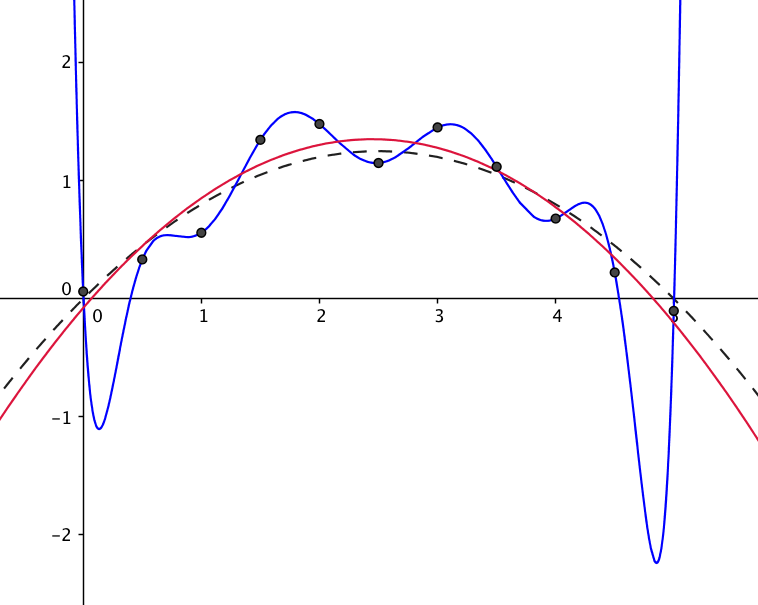
\includegraphics[width="50\%"]{overfitting.png}
    \caption{Fitting a degree $2$ polynomial (in red) and a degree $10$ polynomial (in blue) to the sample data $ \mathcal{D} $. The target function $p$ is the dashed curve. We see that the simple quadratic fit is much closer to the target function and hence performes better on new data.}
  \end{figure}

  In later chapters we will see how the degree $2$ polynomial fit was
  obtained. This is a nice example of a convex
  optimization problem.% called regression.

  \end{document}